% 
% Annual Cognitive Science Conference
% Sample LaTeX Paper -- Proceedings Format
% 

% Original : Ashwin Ram (ashwin@cc.gatech.edu)       04/01/1994
% Modified : Johanna Moore (jmoore@cs.pitt.edu)      03/17/1995
% Modified : David Noelle (noelle@ucsd.edu)          03/15/1996
% Modified : Pat Langley (langley@cs.stanford.edu)   01/26/1997
% Latex2e corrections by Ramin Charles Nakisa        01/28/1997 
% Modified : Tina Eliassi-Rad (eliassi@cs.wisc.edu)  01/31/1998
% Modified : Trisha Yannuzzi (trisha@ircs.upenn.edu) 12/28/1999 (in process)
% Modified : Mary Ellen Foster (M.E.Foster@ed.ac.uk) 12/11/2000
% Modified : Ken Forbus                              01/23/2004
% Modified : Eli M. Silk (esilk@pitt.edu)            05/24/2005
% Modified : Niels Taatgen (taatgen@cmu.edu)         10/24/2006
% Modified : David Noelle (dnoelle@ucmerced.edu)     11/19/2014
% Modified : Roger Levy (rplevy@mit.edu)     12/31/2018



%% Change "letterpaper" in the following line to "a4paper" if you must.

\documentclass[10pt,letterpaper]{article}

\usepackage{cogsci}

%\cogscifinalcopy % Uncomment this line for the final submission 


\usepackage{pslatex}
\usepackage{apacite}
\usepackage{float} % Roger Levy added this and changed figure/table
                   % placement to [H] for conformity to Word template,
                   % though floating tables and figures to top is
                   % still generally recommended!
\usepackage{amsmath}
\usepackage{amssymb}
\usepackage{graphicx}
\usepackage{subcaption}

%\usepackage[none]{hyphenat} % Sometimes it can be useful to turn off
%hyphenation for purposes such as spell checking of the resulting
%PDF.  Uncomment this block to turn off hyphenation.


%\setlength\titlebox{4.5cm}
% You can expand the titlebox if you need extra space
% to show all the authors. Please do not make the titlebox
% smaller than 4.5cm (the original size).
%%If you do, we reserve the right to require you to change it back in
%%the camera-ready version, which could interfere with the timely
%%appearance of your paper in the Proceedings.



\title{How the Teaching Style and Interpretation Type of State Interventions Shape Multi-Agent Coordination}
 
\author{{\large \bf To fill in (email here)} \\
  address line 1 \\
  address line 2
  \AND {\large \bf author 2 (email here)} \\
  address line 1 \\
  address line 2}

\begin{document}

\maketitle


\begin{abstract}
How can an external teacher accelerate coordination among multiple learning agents? We investigate this question in a multi-agent foraging task where a simulated teacher can physically relocate agents—a direct but ambiguous pedagogical signal. We formalize a taxonomy of teaching styles (e.g., \emph{Undoing}, \emph{Correcting}) and agent interpretation rules. Our computational experiments reveal that the \textbf{\emph{Undoing} style is a uniquely powerful catalyst for spatial coordination}, most effectively breaking behavioral symmetry between two agents by imposing spatial constraints that define ``home regions.'' This catalytic effect scales, reinforcing niche specialization in three-agent systems. However, success is governed by a \textbf{pedagogical matching principle}: interventions fail when the agent's interpretation rule mismatches the teacher's intent (e.g., \emph{Correcting} fails when interventions are interpreted as punitive). Our work provides a formal framework showing how structured guidance and agent interpretation jointly shape the emergence of collective organization.

\textbf{Keywords:} Multi-agent reinforcement learning; pedagogy; state intervention; coordination; spatial specialization.
\end{abstract}

\section{Introduction}

Teaching in complex, dynamic environments often extends beyond verbal instruction to include direct manipulation of the learner's state. In multi-agent settings, the challenge of such pedagogical intervention intensifies: the teacher must guide individual learning while fostering collective coordination under real-time resource competition. While previous research has explored how agents interpret physical corrections in single-agent tasks, the role of state interventions as a tool for shaping group-level behavior remains under-explored.

This paper investigates a core computational question: \textbf{How can different algorithmic teaching styles---defined by when and where an agent is moved---catalyze and stabilize spatial coordination in multi-agent systems?} Unlike traditional reinforcement learning where coordination emerges slowly from self-interested exploration, we treat state intervention as a form of fast, asymmetric environmental shaping. We specifically examine how interventions can break the initial behavioral symmetry between agents, leading to \textit{spatial specialization}---a division of labor that minimizes competitive overlap.

The complexity of this teaching scenario is defined by delayed pedagogical outcomes and the teacher's need to manage multiple agents under spatial uncertainty. Rather than focusing on the agent's internal interpretive ambiguity, we adopt a \textbf{system-level modeling approach} to map the performance landscape across various teaching styles and agent interpretation rules.

To our knowledge, this is the first systematic investigation of state interventions in real-time, multi-agent, discrete environments where the teacher lacks access to the learner's feature representation. By bridging the gap between heuristic pedagogical strategies and multi-agent coordination, our work provides a computational foundation for designing adaptive agents that learn effectively from structured external guidance. Our contributions are as follows:

\begin{itemize}
    \item We formalize a taxonomy of algorithmic teaching styles designed to shape multi-agent coordination through state interventions.
    \item We identify a \textbf{pedagogical matching principle}, demonstrating that the effectiveness of an intervention depends on the alignment between the teaching strategy and the agents' interpretation rules.
    \item We demonstrate that specific interventions act as uniquely powerful catalysts for symmetry breaking and stable spatial niche formation.
\end{itemize}

\section{Prior work}

Our work sits at the intersection of computational models of teaching, reinforcement learning from human feedback, and multi-agent systems. This section provides an overview of the relevant literature along these axes, highlighting how our approach diverges from and extends prior research.

\subsection{Computational Models of Teaching and Intervention}

Formal models of teaching often build upon the framework of Partially Observable Markov Decision Processes (POMDPs) to capture the interactive dynamics between a teacher and a learner~\cite{kaelbling1998}. This formalism has been productively applied to understand human pedagogical reasoning~\cite{shafto2014} and to design algorithms for efficient instruction~\cite{rafferty2016}. A key insight from this line of work is that teaching is not merely reinforcement; it is a communicative act where signals are chosen to influence the learner's beliefs and future behavior~\cite{ho2019people, ho2021}.

Within this broad context, \emph{physical state intervention} represents a particularly direct yet ambiguous teaching signal. Early computational work by~\citeA{ho2017} explored how people use interventions to guide an agent to a goal while avoiding obstacles, framing the problem as one of inferring the teacher's intent from physical corrections. More recently,~\citeA{losey2022physical} formalized physical human-robot interaction as a POMDP where the robot maintains a belief over the human's unknown reward function, that is updated through physical corrections interpreted as intentional signals. Their work demonstrates that heuristic interpretations of interventions (e.g., updating one feature weight at a time) can improve learning efficiency. However, these approaches are designed for \textbf{single-agent, continuous-control tasks} (e.g., robotic manipulation) and assume a \textbf{shared, known feature space} between human and robot, which allows for a relatively straightforward mapping from physical corrections to reward function updates.

In contrast, our work investigates discrete grid-based environments where agents learn \emph{tabula rasa} via model-free RL without prior knowledge of task features or reward structure. The teacher's interventions (e.g., dragging an agent to a new tile) must therefore be interpreted through heuristic rules defined at the level of state transitions and value updates, not feature-weight adjustments. We extend the idea of heuristic interpretation by proposing and systematically evaluating a broader taxonomy of such rules.

\subsection{Reinforcement Learning from Human Feedback and Guidance}

The paradigm of Reinforcement Learning from Human Feedback (RLHF) and related interactive techniques provide a rich foundation for learning from various forms of human input~\cite{luo2024precise}. In such frameworks, human interventions are often treated as demonstrations or preference labels. For instance,~\citeA{luo2024precise} treat human interventions during high-dimensional manipulation tasks as \emph{suggestions}, where the agent learns directly from the state-action pair induced by the human.

A crucial distinction in our setting is the nature of the task and agent embodiment. Unlike continuous control tasks where a human can kinesthetically guide an end-effector through a physically plausible trajectory, our discrete environment introduces a fundamental asymmetry: the teacher can \emph{teleport} an agent to any tile. An action the agent cannot replicate on its own. This breaks the direct \emph{"suggestion as demonstratable action"} assumption common in RLHF for robotics. Consequently, we must consider interpretations beyond direct imitation, such as treating an intervention as a reset, an interruption, or even a punitive signal.

\subsection{Multi-Agent Learning and the Role of External Shaping}

In multi-agent reinforcement learning (MARL), coordination often emerges from self-interested learning \cite{axelrod1984cooperation, austerweil2015impact} or is engineered through specific reward structures \cite{wolpert2001optimal} and communication protocols \cite{foerster2016learning}. External shaping by a teacher adds a new dimension to this problem. While there is extensive literature on centralized training for decentralized execution \cite{lowe2017multi, rashid2020monotonic, foerster2018counterfactual} and on learning communication protocols \cite{foerster2016learning}, the explicit study of how \textbf{an external teacher can use state interventions to shape multi-agent coordination} is nascent.

Classic game-theoretic analyses show that cooperation can emerge in repeated interactions without explicit social motivations~\cite{axelrod1984cooperation}, and self-interested agents can discover cooperative strategies in many grid-world games~\cite{austerweil2015impact}. However, analyzing two or more agents with continuous-time, interactive signals remains open. Our work investigates whether and how targeted state interventions (a form of fast, asymmetric environmental shaping) can accelerate and stabilize the emergence of coordinated behaviors, such as spatial division of labor, in a learning population. This connects to broader questions in social learning about how environmental structure mediates the value of external information~\cite{wu2025adaptive}. We contribute by providing a formal framework to study this specific shaping mechanism.

\section{Method}

We investigate a real-time foraging task in a discrete grid world. A fixed set of tiles are designated as spawn tiles, where pellets appear stochastically over time following a Poisson process~\cite{kingman1992}. We focus on a \emph{smooth} distribution, where spawn tiles are grouped into a small number of contiguous, spatially coherent regions~\cite{wu2025adaptive}. Agents occupy a single tile and move continuously toward adjacent tiles (including diagonals) over a fixed duration. When an agent overlaps with a pellet, it receives a reward $R_{\text{pellet}}$ and the pellet is consumed.

A \emph{simulated teacher} with perfect knowledge of the spawn distribution (but not real-time pellet presence) can perform \emph{state interventions}: forcibly relocating an agent to a new tile at any moment. The agent then resumes its policy from this new state. The teacher decides when to intervene by estimating, for each possible action an agent could take from its current position, the long-term value of that action based solely on the known spawn distribution. If the agent's chosen action is estimated to be suboptimal (i.e., less valuable than the best available alternative from that position), the teacher triggers an intervention with a probability specified by the \emph{intervention rate} parameter. The intervention itself is determined by the \emph{teaching style}.

This setup introduces several learning challenges: (1) rewards are dynamic and stochastic; (2) agents learn online via reinforcement learning with no prior knowledge; (3) we analyze systems involving \textbf{two or three agents} operating concurrently, which creates competitive pressure and requires spatial coordination; (4) interventions provide an ambiguous, real-time pedagogical signal that agents must interpret within these multi-agent social dilemmas. Together, these features create a complex testbed for evaluating how pedagogical interventions can effectively guide agents toward collective coordination and mitigate competition in dynamic environments.

\subsection{Intervention styles}

Our environment is modeled as a Markov Decision Process (MDP) $\left(S, A, T, R, \gamma \right)$, where the state space $S$ corresponds to the agent's discrete grid position; the action space $A$ includes movements to the eight adjacent tiles; the transition function $T$ is deterministic; the immediate reward $R(s_t, a_t, s_{t+1})$ is stochastic, depending on whether a pellet is collected during the movement from $s_t$ to $s_{t+1}$; and $\gamma$ is the discount factor.

Agents learn via Q-learning \cite{suttonbarto2018} with an $\epsilon$-greedy policy. The standard Q-update given a transition $(s_t, a_t, s_{t+1}, r_t)$ is:
\begin{equation}
Q(s_t,a_t) \leftarrow Q(s_t,a_t) + \alpha \left[r_t + \gamma \max_{a'} Q(s_{t+1},a') - Q(s_t, a_t) \right]
\end{equation}

A core challenge is how an agent should update its value function when its movement is interrupted by a state intervention. We formalize this by distinguishing between:
\begin{itemize}
    \item $s^A_{t+1}$: the state the agent would have reached autonomously,
    \item $s^I_{t+1}$: the agent's state post-intervention,
    \item $a_t$: the original action attempted by the agent,
    \item and $r_t$: any environmental reward received up to the point of interruption.
\end{itemize}
We also define $a^I$ as the action from $s_t$ that minimizes Euclidean distance to $s^I_{t+1}$, and $r^I$ as the reward obtained at $s^I_{t+1}$.
\begin{figure}[htbp]
    \centering
    \includegraphics[width=0.3\linewidth]{figs/interpretation.png}
    \caption{As an agent moves along the red arrow (action $a_t$) moving from the black ($s_t$) to red tile ($s^{A}_{t+1}$), it is intervened on and is placed on the blue tile ($s^I_{t+1}$). The blue arrow $a^I$ is the closest action from the starting black tile $s_t$ the post-intervention blue tile $s^I_{t+1}$.}
    \label{fig:interpretation}
\end{figure}
To systematically evaluate these interpretation types, we define four algorithmic \textbf{teaching styles} that determine \emph{when} and \emph{where} to intervene:
\begin{itemize}
    \item \textbf{Undoing}: Returns the agent to its previous state $s_t$.
    \item \textbf{Correcting}: Moves the agent to a randomly selected pellet spawn tile within a $5\times5$ neighborhood of $s_t$.
    \item \textbf{Exploration-encouraging Correcting}: Moves the agent to a non-spawn tile adjacent (within a $3\times3$ area) to a spawn tile in the $5\times5$ neighborhood of $s_t$.
    \item \textbf{Restart}: Moves the agent to a non-spawn tile in the $5\times5$ neighborhood of $s_t$, far from any spawn tile.
\end{itemize}
An intervention is triggered probabilistically (via an \textit{intervention rate} parameter) when the agent's current action is estimated to be suboptimal relative to the known spawn tile distribution.

\subsection{Intervention Interpretation}

How should an agent update its value function when its movement is interrupted by a state intervention? When externally displaced, an agent must infer the pedagogical intent behind the intervention. We propose six distinct \textbf{interpretation types} for mapping an intervention event to a Q-update:

\begin{itemize}
    \item \textbf{Suggestion}: Treats $s^I_{t+1}$ as a recommended goal. \textit{Update:} $(s_t, a^I, s^I_{t+1}, r^I)$.
    \item \textbf{Reset}: Treats intervention as a neutral relocation adapted from \cite{ho2017}. \textit{Update:} $(s_t, a_t, s^A_{t+1}, r_t)$.
    \item \textbf{Interrupt}: Treats intervention as a mere interruption adapted from \cite{ho2017}. No Q-update is performed.
    \item \textbf{Transition}: Treats intervention as a positive guided transition. \textit{Update:} $(s_t, a^I, s^I_{t+1}, +2R_{\text{pellet}})$. If $s^I_{t+1}=s_t$, it is treated as negative: $(s_t, a_t, s^A_{t+1}, -2R_{\text{pellet}})$.
    \item \textbf{Disrupt}: Treats any intervention as inherently negative. \textit{Update:} $(s_t, a^I, s^I_{t+1}, -2R_{\text{pellet}})$.
    \item \textbf{Impede}: Treats intervention as a punishment for the original action. \textit{Update:} $(s_t, a_t, s^A_{t+1}, -2R_{\text{pellet}})$.
\end{itemize}

\noindent These interpretation types represent distinct computational hypotheses for how physical interventions function as communicative acts within the learning process.

\subsection{Policy Evaluation and Coordination Metrics}

The stochastic and dynamic nature of pellet generation, and multi-agent interaction violates the standard Markov assumption. Explicitly modeling pellet counts would lead to a combinatorial state explosion. Therefore, to evaluate and compare policies, we approximate the \textbf{expected reward} of a policy $\pi$ through simulation:
\begin{equation}
    \hat{V}(\pi) = \frac{1}{100} \sum_{k=1}^{100} \sum_{\tau=0}^{30} \gamma^\tau r^{(\tau)}_{k},
\end{equation}
where $r^{(\tau)}_{k}$ is the reward obtained at step $\tau$ in the $k$-th rollout. Each rollout starts the agent from a random position and executes $\pi$ for 30 steps in a new environment instance (with other agents). This metric estimates the agent's average foraging efficiency under environmental and interactive stochasticity.

To systematically map the multi-agent coordination landscape, we perform a factorial analysis across the proposed taxonomy of \emph{teaching styles} and \emph{interpretation types}. This approach allows us to investigate how specific combinations of pedagogical signals and agent-level heuristics interact with environmental topology. By evaluating these configurations in spatially continuous ``smooth'' environments, we aim to identify the computational conditions that yield the most stable policy acquisition and group-level performance.

Coordination emerges as a critical computational challenge, when the multi-agent system scales. Ideally, agents should minimize competitive overlap by partitioning the environment—a phenomenon we term \textit{spatial specialization}. The goal is to investigate how intervention styles act as a catalyst for this coordination, specifically examining whether structured interventions can break the initial behavioral symmetry between agents.

\section{Results and Analysis}

\begin{figure}[htbp]
    \centering
    \begin{subfigure}[b]{\linewidth}
        \centering
        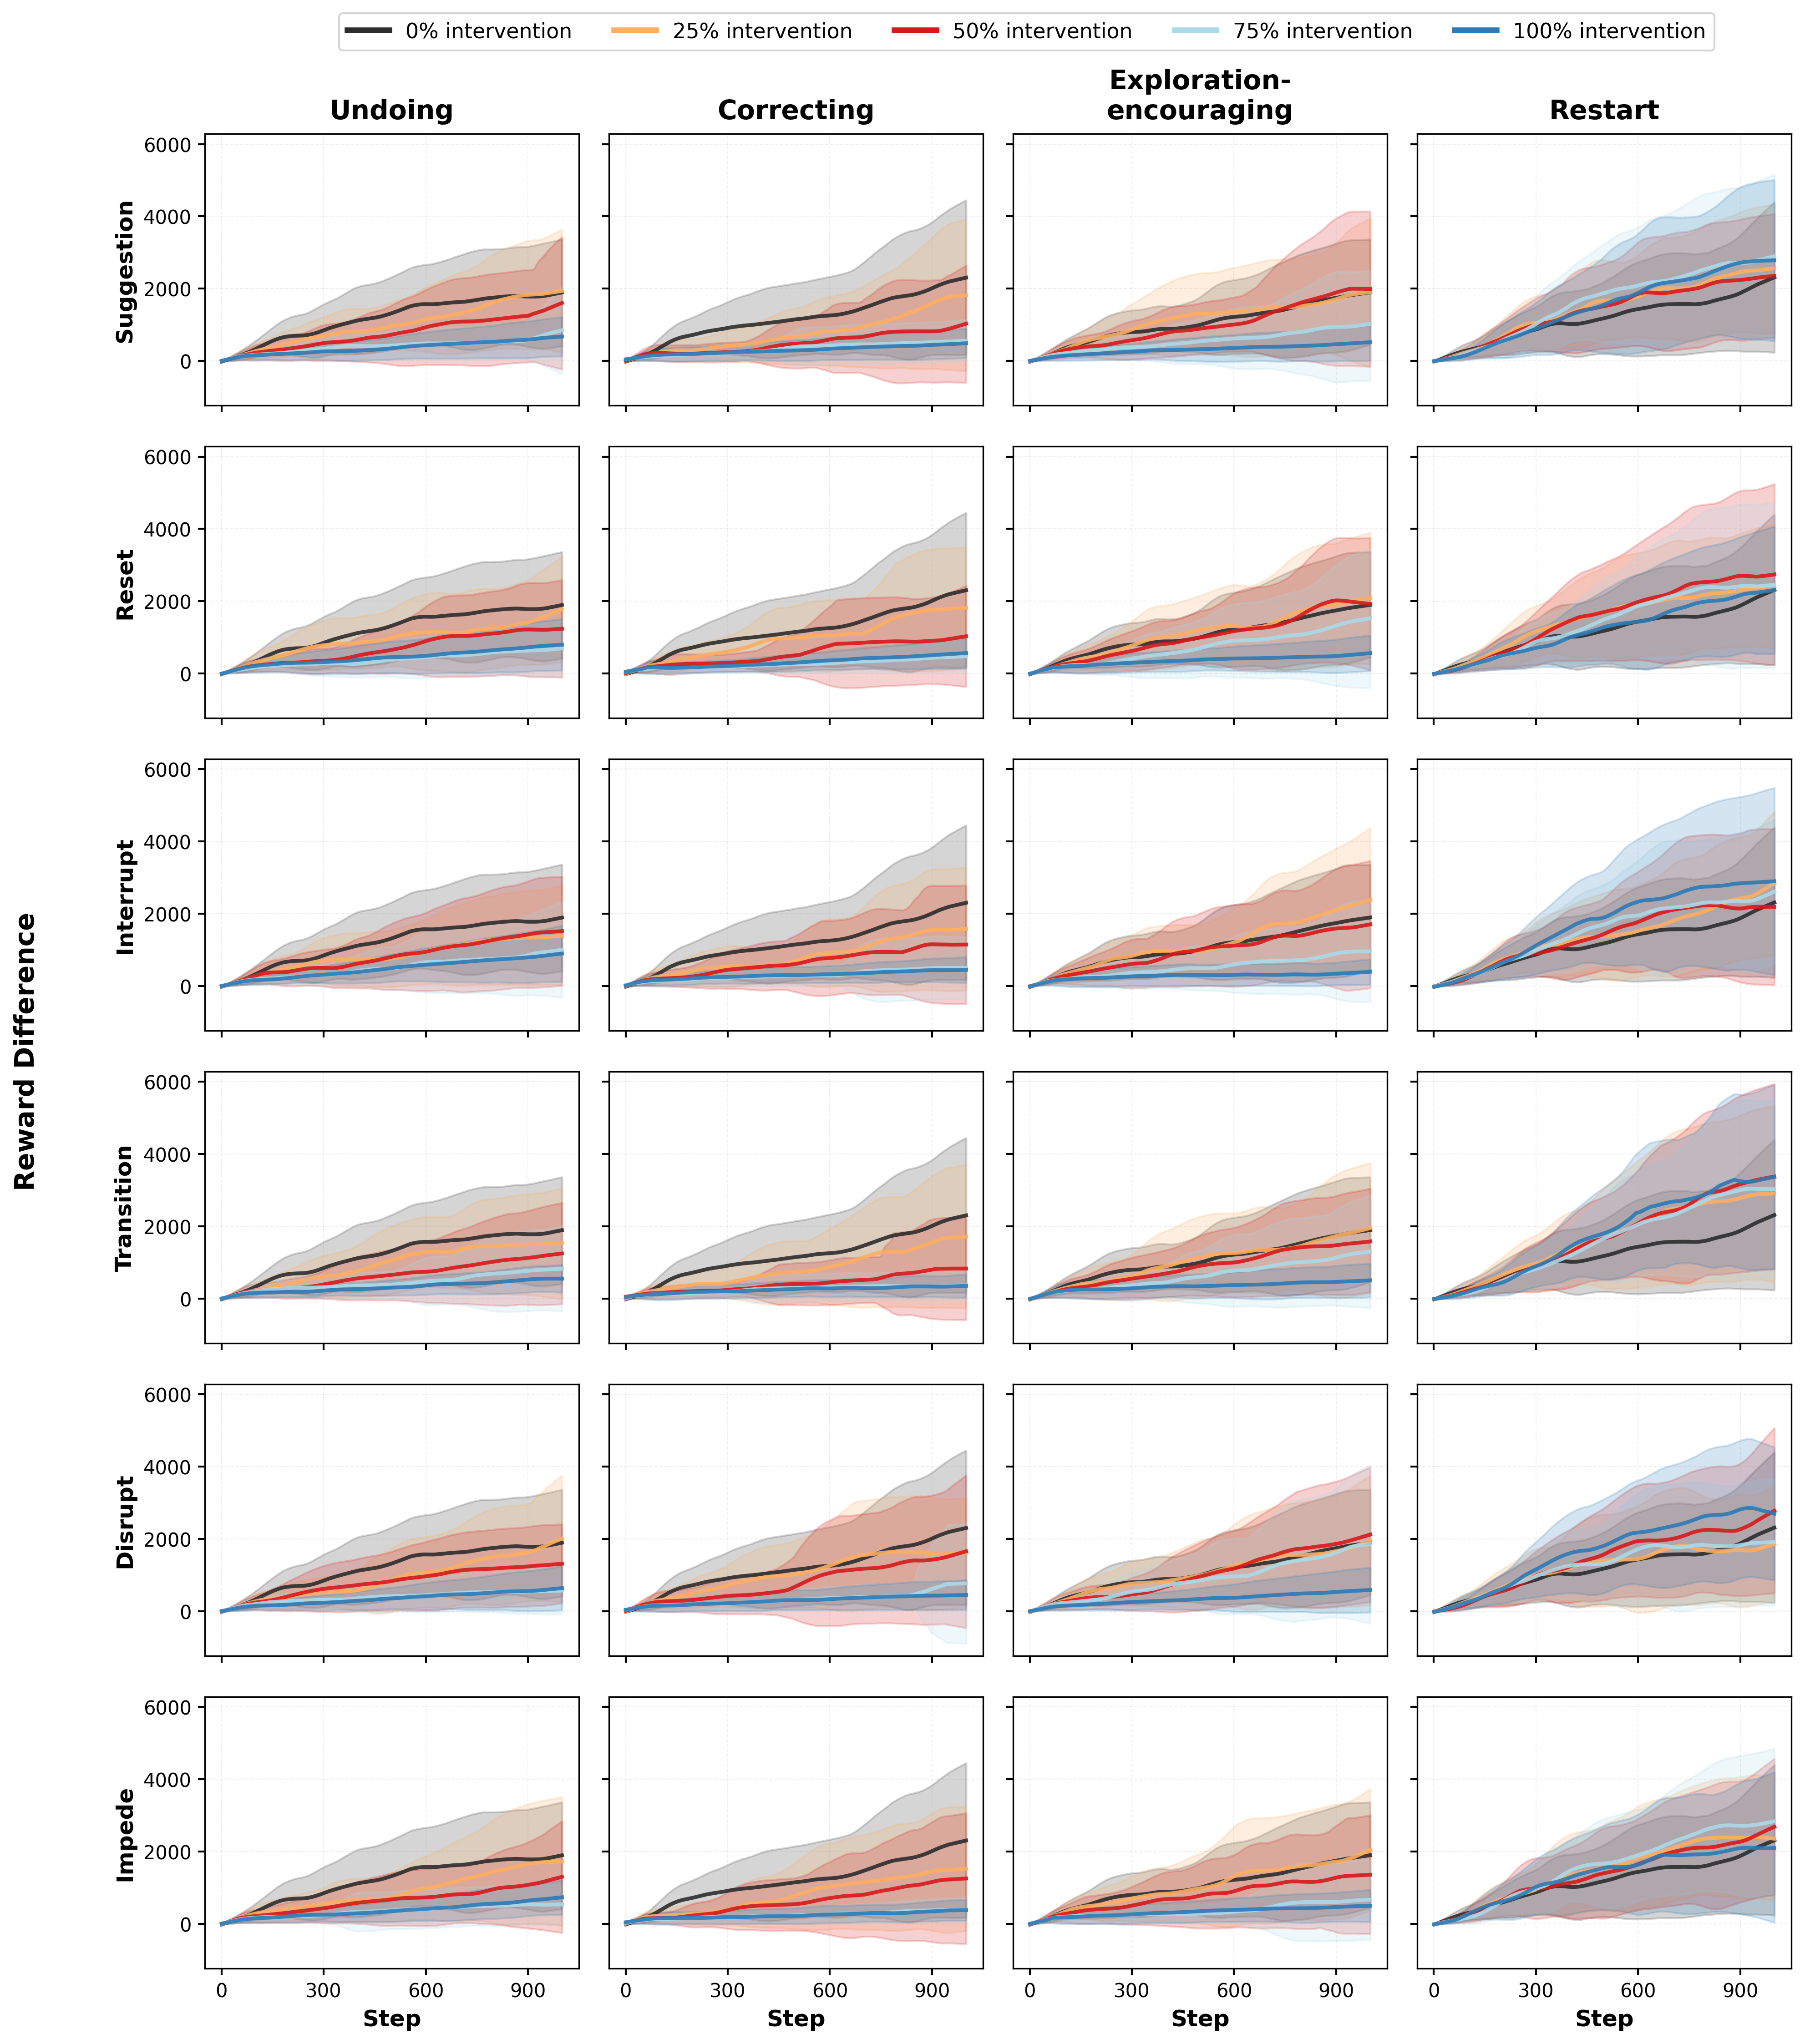
\includegraphics[width=\textwidth]{figs/n6.2.21.png}
        \caption{Policy Divergence. Larger values reflect better coordination.}
        \label{fig:6.2.21}
    \end{subfigure}
    \begin{subfigure}[b]{\linewidth}
        \centering
        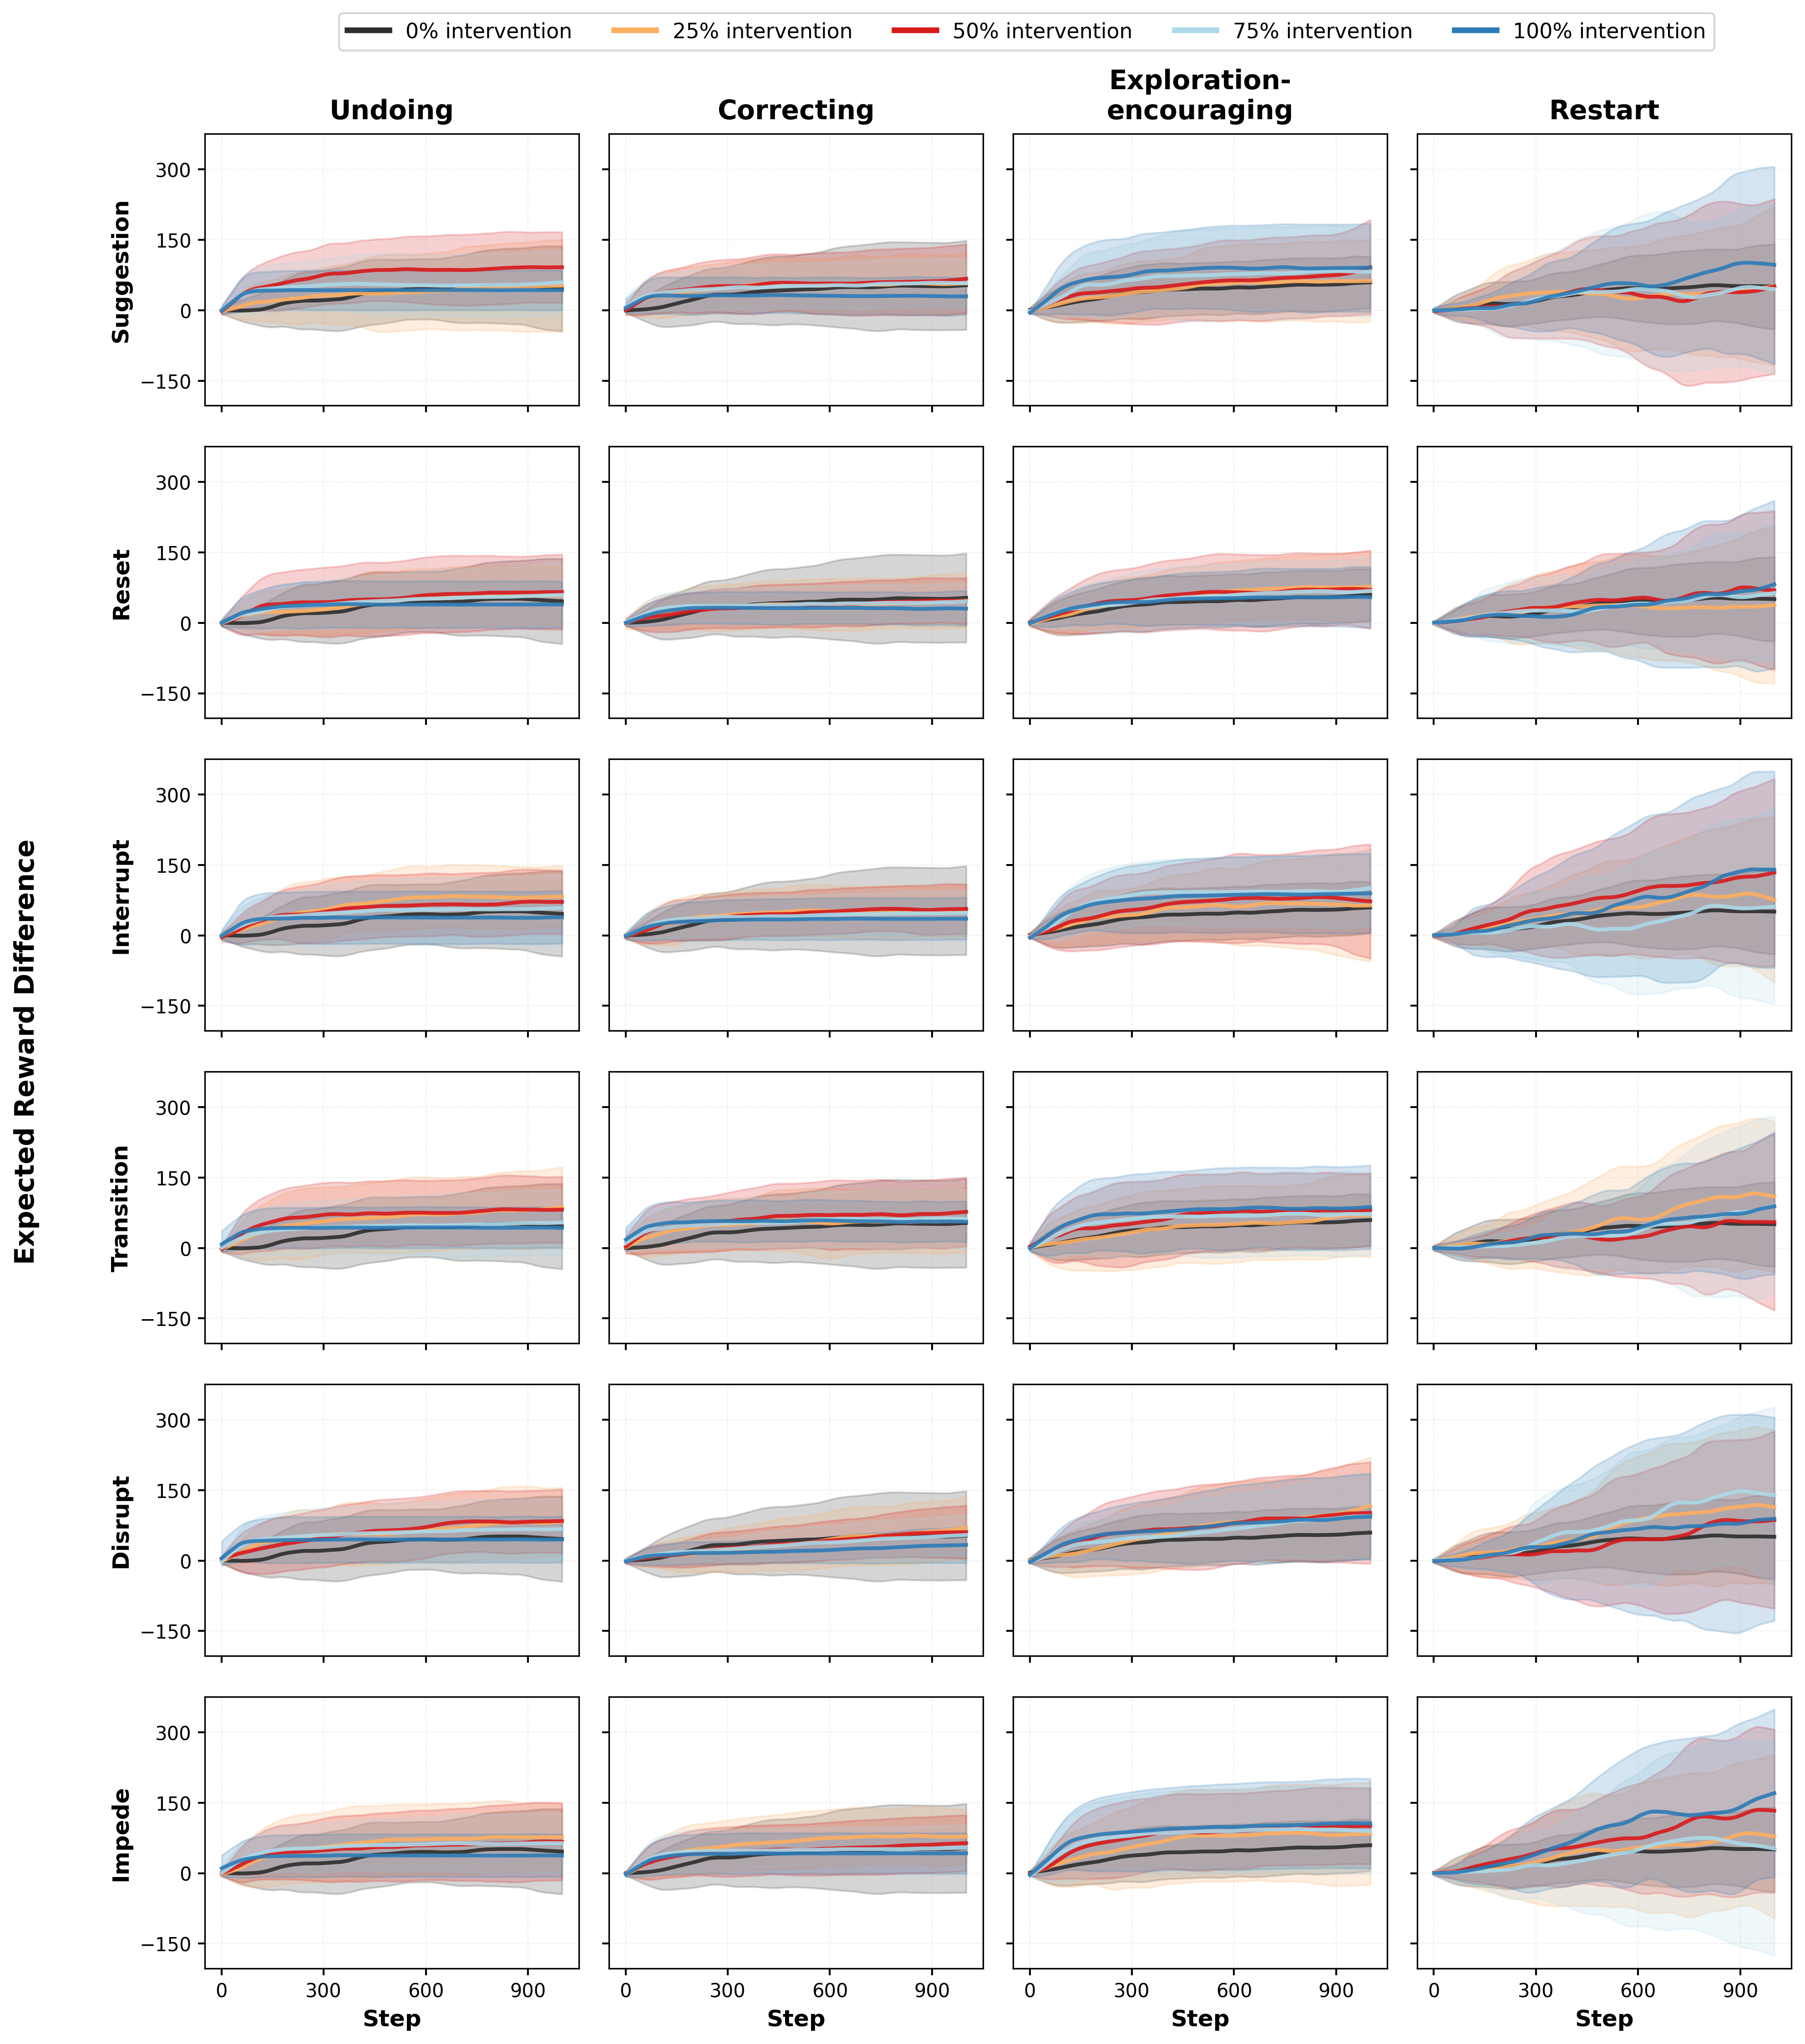
\includegraphics[width=\textwidth]{figs/n6.2.22.png}
        \caption{System Equilibrium. Smaller values reflect greater fairness.}
        \label{fig:6.2.22}
    \end{subfigure}
    
    \caption{Policy Divergence and System Equilibrium for Two-Agent Experiments. Rows and columns vary in intervention interpretations and teaching styles, respectively. The intervention rates are color-coded as follows: 0 (black), 0.25 (light red), 0.5 (red), 0.75 (light blue), and 1 (blue). An appropriate teaching style can accelerate the coordination among agents, allowing each agent to focus on a specific region and achieve balanced scoring.}
    \label{fig:6.2.2}
\end{figure}

\subsubsection{Emergence of Coordination in Two-Agent Systems}
We measure \textit{coordination} through two metrics: 
(1) \textbf{Policy Divergence}: The degree to which agents specialize in different regions, measured by the difference in their ``first-region preference'' (Expected Reward in Region 1 minus Region 2).
(2) \textbf{System Equilibrium}: The balance of resource acquisition, measured by the absolute score difference between agents.

In an environment with two regions, Figures~\ref{fig:6.2.21} and \ref{fig:6.2.22} reveal that the \textit{Undoing} style as the most robust style for policy divergence and system equilibrium.  All teaching styles provide benefits for policy divergence. However, \textit{Correcting} strategies require large intervention rates ($\geq0.75$) to support policy divergence and system equilibrium early. \textit{Restart} discourages system equilibrium.  By forcibly resetting an agent's state when it encroaches on suboptimal or redundant paths, \textit{Undoing} effectively balances both policy divergence and system equilibrium (though higher intervention rates, $\geq0.75$ are still needed for this).

%increases the computational cost of competitive overlap. We found that an intervention rate of 0.5 is the ``sweet spot'' for maximizing policy divergence; however, higher rates ($\geq0.75$) are required to maintain a balanced system (stable scores). 
%The \textit{Exploration-encouraging Correcting} style can also serve as a catalyst for early symmetry breaking, but it requires a higher intervention rate ($\lambda > 0.75$) to achieve significant effects. This is especially evident in the system equilibrium metric: without a high intervention rate, agents maintain a differentiated division of labor only theoretically (at the policy divergence level), but not in practice. This suggests that when encouraging agents to explore, the teacher must provide more frequent "boundary interventions" to prevent them from reentering each other's spatial niches.

% In contrast, the \textit{Correcting} style facilitates rapid initial coordination but often fails to reach a stable state of complete specialization. Notably, the \textit{Restart} style acted as a disruptor, frequently resetting progress and widening the scoring gap between agents, thereby failing to support consistent coordination.

Examining the \emph{interpretation types} of agents, \textit{Reset} performs poorly across most \emph{teaching styles}. \textit{Disrupt} is less compatible with the \textit{Correcting} style, where pedagogical interventions consistently undermine the differentiation of labor. This suggests that in coordination tasks, agents should attempt to align with the most direct interventions rather than interpreting them as negative signals. It also suggests that overly direct corrections should not be applied to such agents.

\subsubsection{Niche Reinforcement in Three-Agent Systems}
\begin{figure}[htbp]
    \centering
    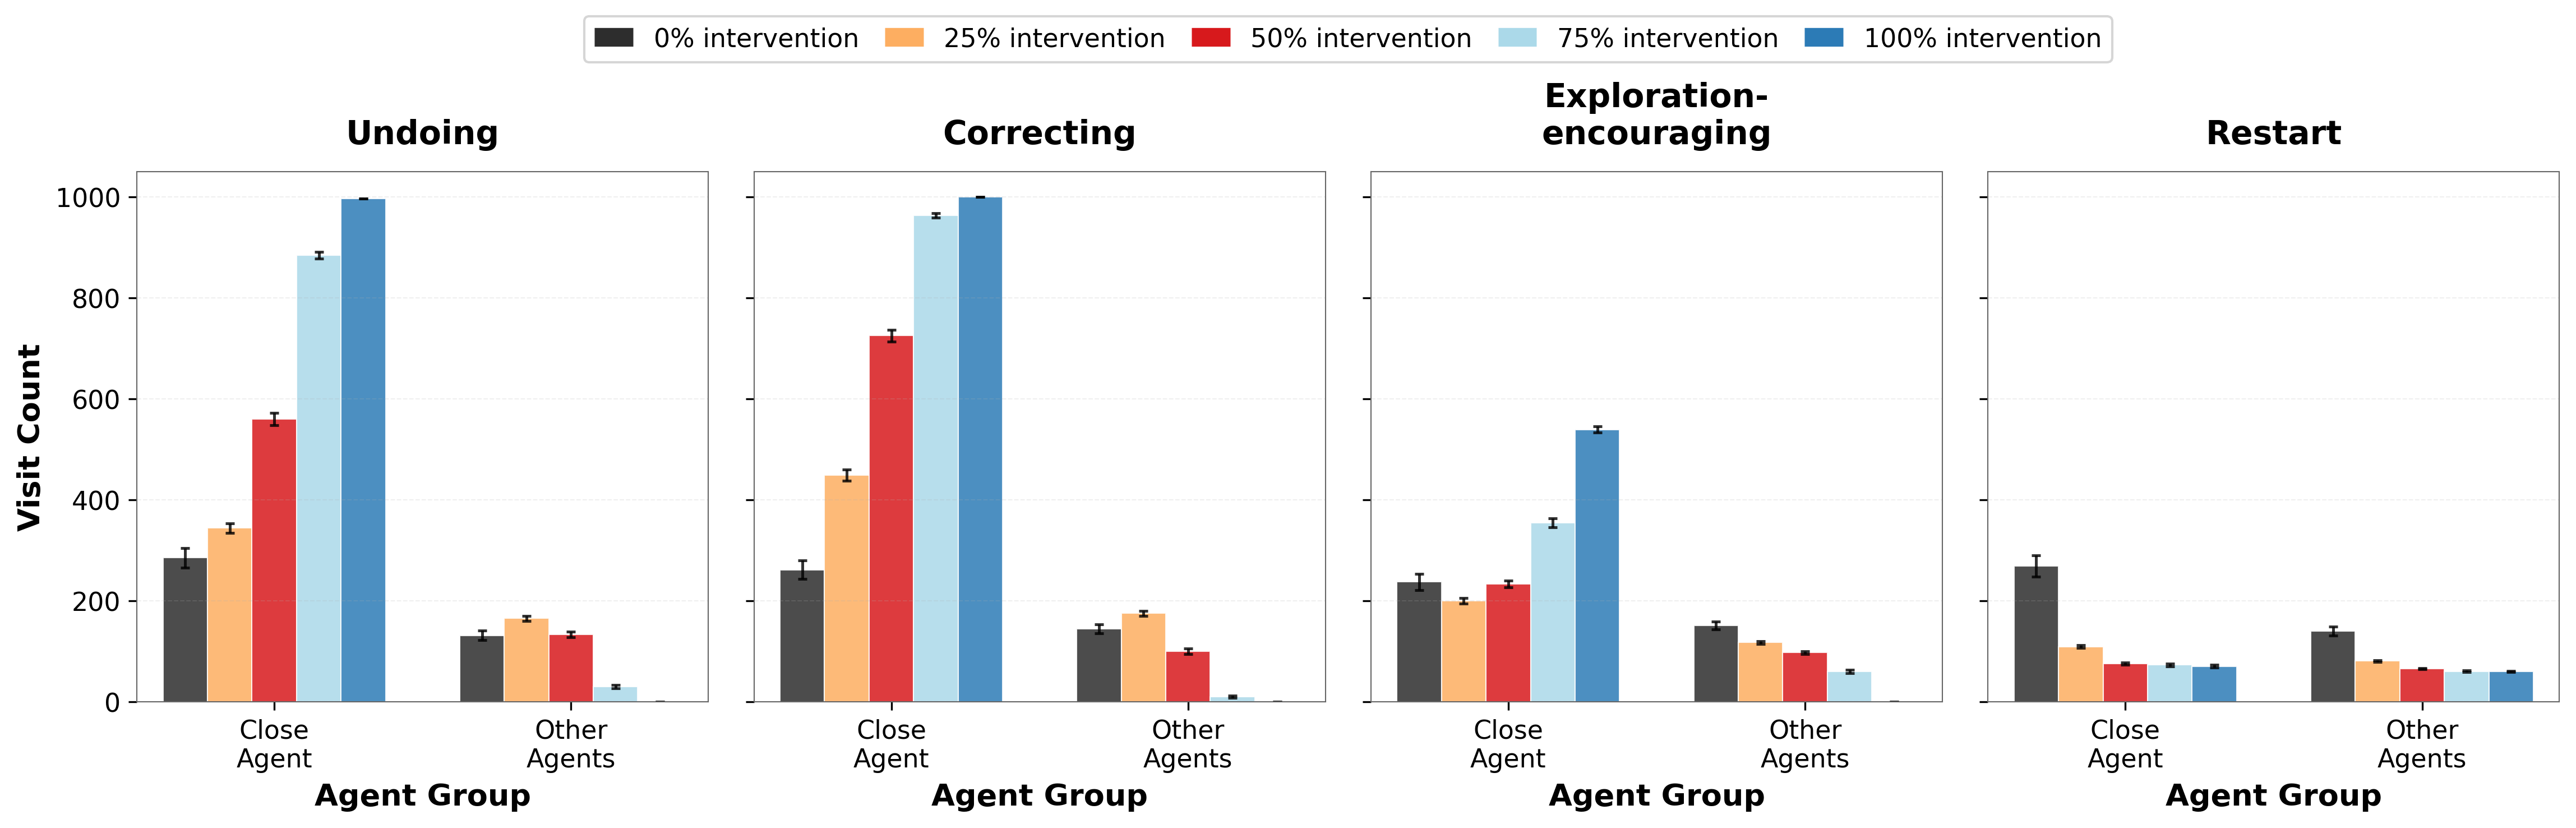
\includegraphics[width=1\linewidth]{figs/6.2.1.png}
    \caption{Three-agent simulation results. Visit count of agents for different teaching styles. Color denotes intervention rate: 0 (black), 0.25 (light red), 0.5 (red), 0.75 (light blue), and 1 (blue). An appropriate teaching style can enhance the coordination among multiple agents.}
    \label{fig:6.2.1}
\end{figure}
In an environment with three regions and three agents, Figure~\ref{fig:6.2.1} illustrates the visit count of agents to their closest regions. Both \textit{Undoing} and \textit{Correcting} styles significantly amplified the \textit{spatial attachment} of agents and encouraged coordination more robustly than other teaching styles. As the intervention rate increased, we observed a linear strengthening of niche persistence across all interpretation types. This indicates that these styles function as a \textit{positive feedback loop} for coordination: by correcting local errors, the teacher implicitly solidifies the agent's role within the emerging spatial division of labor.

The \textit{Exploration-encouraging Correcting} style produced a more diffused spatial footprint; while agents remained primarily in their assigned regions, they exhibited a higher probability of cross-regional foraging. This confirms that this style prioritizes individual policy robustness over strict group coordination. The \textit{Restart} style again proved detrimental, actively dismantling the spatial niches and leading to chaotic, uncoordinated foraging patterns.

\section{Discussion}

This study systematically explores how algorithmic teaching styles, mediated by agent interpretation rules, can catalyze spatial coordination in multi-agent reinforcement learning. Our central finding is that the \textbf{\emph{Undoing} intervention style serves as a uniquely powerful catalyst for multi-agent coordination}, most effectively breaking behavioral symmetry between two agents. The overall effectiveness of pedagogical intervention, however, is governed by a \textbf{pedagogical matching principle}: successful coordination requires coherence between the teacher's external action and the learner's internal heuristic. Our results provide concrete evidence for this principle by revealing critical \emph{mismatches}. The \emph{Reset} interpretation consistently led to poor performance across all teaching styles, indicating a universal failure to align with pedagogical intent. More specifically, a severe mismatch occurred when agents using the \emph{Disrupt} interpretation (viewing all interventions as negative) were subjected to the \emph{Correcting} style, which actively undermined the very coordination it aimed to promote.

Crucially, the coordination-promoting effect of appropriate teaching scales to more complex multi-agent societies. In three-agent systems, both \emph{Undoing} and \emph{Correcting} styles robustly reinforced the emerging spatial niches, significantly increasing agents' attachment to their primary regions. This demonstrates that targeted state interventions can transcend simple pairwise coordination and act as a \textit{positive feedback loop} that solidifies collective organization. The failure of the \emph{Restart} style across both two- and three-agent scenarios further underscores that not all interventions are helpful; pedagogical success requires the external guidance to be structured in a way that is computationally interpretable and aligned with the goal of reducing competitive overlap.

These requirements for interpretability and goal alignment are met by the distinct pedagogical policies that our teaching styles operationalize. The \emph{Undoing} style, which forcibly returns the agent to its previous state, emerged as a uniquely powerful catalyst for multi-agent coordination. Its efficacy does not stem from conveying a specific reward or penalty, but from imposing a strong \emph{spatial constraint}. By repeatedly resetting an agent's position, it effectively defines a ``home region'' and increases the cost of venturing into areas dominated by others. This mechanism rapidly breaks behavioral symmetry and enforces spatial niche formation---a crucial step in solving the ``clash of interests'' in collective learning. This finding demonstrates how structured external intervention can \emph{accelerate and stabilize} the emergence of cooperative equilibria that self-interested learners might otherwise discover slowly or unreliably \cite{austerweil2015impact}.

Conversely, the \emph{Correcting} style functions more as a \textbf{stabilizing force}. Once a basic spatial division has emerged, \emph{Correcting} is sufficient to reinforce these existing niches by guiding agents back to their respective optimal regions without the high cost of total displacement.

However, its effectiveness as a stabilizer is contingent upon the agent's interpretation, as evidenced by its severe incompatibility with the \emph{Disrupt} rule. This observation refines the pedagogical matching principle: a well-intentioned guiding correction can fail if the learner misinterprets it as a cautionary demonstrations.

Together, these insights suggest a potential trajectory for adaptive pedagogical systems: transitioning from symmetry-breaking interventions (\emph{Undoing}) to refinement-oriented guidance (\emph{Correcting}) as the multi-agent system matures, while remaining mindful of the agents' evolving interpretative frameworks.


\subsection{Future Work}
The current study establishes that state interventions, particularly the \emph{Undoing} style, can act as a powerful catalyst for spatial coordination under specific conditions (smooth resource distributions, tabula rasa learners). A critical trajectory for future research lies in testing the boundary conditions and generalizability of these effects by introducing greater ecological complexity.

First, transitioning from fully observable grid worlds to Partially Observable Markov Decision Processes (POMDPs) would introduce realistic perceptual uncertainty. In such settings, state interventions could function not only as spatial corrections but also as \emph{information-shaping signals} that reduce a learner's belief entropy about the reward landscape. The teacher's role would thus evolve from trajectory correction to active epistemic guidance, where interventions like \emph{Undoing} might serve to prune sub-optimal hypotheses or direct attention. Exploring whether the catalytic effect of \emph{Undoing} persists, or how the required \textbf{pedagogical matching} between style and interpretation changes under partial observability, is a key next step.

Second, the robustness of our identified mechanisms across different environmental structures remains to be explored. For instance, would \emph{Undoing} remain the dominant catalyst in environments with fragmented or dynamically shifting resources? Investigating how the effectiveness of different teaching styles varies with environmental topology will clarify the scope of our findings and inform the design of context-aware pedagogical agents.

Furthermore, the scalability and inherent heterogeneity of multi-agent systems present a vital frontier. Beyond the small, homogeneous groups explored here, larger populations introduce complex collective dynamics with diverse learning rates, sensory capabilities, or intrinsic motivations. Future work should focus on how a teacher (centralized or distributed) can use state interventions to manage such a ``heterogeneous classroom''—enforcing specialization, preventing maladaptive cascades, and maintaining a robust socio-technical equilibrium. This entails understanding how to balance individual learning efficiency with global stability as the system scales.

Ultimately, such research is essential for designing adaptive autonomous systems capable of learning and cooperating effectively from structured guidance in high-stakes, real-world environments.

\bibliographystyle{apacite}

\setlength{\bibleftmargin}{.125in}
\setlength{\bibindent}{-\bibleftmargin}

\bibliography{CogSci_Template}
\appendix

%%%%%%%%%%%%


\end{document}
